\documentclass[11pt,a4paper]{article}

% ------------------------------------------------------------------ paquets
\usepackage[utf8]{inputenc}
\usepackage[T1]{fontenc}
\usepackage[french]{babel}
\usepackage{lmodern}
\usepackage{microtype}
\usepackage[margin=2.4cm]{geometry}
\usepackage{amsmath, amssymb}
\usepackage{icomma}
\usepackage{graphicx}
\usepackage{booktabs}
\usepackage{makecell}
\usepackage{float}
\usepackage[font=small,labelfont=bf]{caption}
\usepackage{enumitem}
\usepackage{xcolor}
\usepackage{fancyhdr}
\usepackage{algorithm}
\usepackage[noend]{algpseudocode}
\usepackage[hidelinks]{hyperref}

\graphicspath{{../results/figures/}}
\AtBeginDocument{\renewcommand{\tablename}{Tableau}}

% ---------------------------------------------------------------- couleurs
\definecolor{BleuFonce}{HTML}{0B3D6B}
\definecolor{GrisMoyen}{HTML}{898781}

% -------------------------------------------------------------- algorithmes
\floatname{algorithm}{Algorithme}
\algrenewcommand\algorithmicrequire{\textbf{Entrées :}}
\algrenewcommand\algorithmicensure{\textbf{Sortie :}}
\algrenewcommand\algorithmicfor{\textbf{pour}}
\algrenewcommand\algorithmicforall{\textbf{pour tout}}
\algrenewcommand\algorithmicdo{\textbf{faire}}
\algrenewcommand\algorithmicwhile{\textbf{tant que}}
\algrenewcommand\algorithmicif{\textbf{si}}
\algrenewcommand\algorithmicthen{\textbf{alors}}
\algrenewcommand\algorithmicelse{\textbf{sinon}}
\algrenewcommand\algorithmicreturn{\textbf{retourner}}
\algrenewcommand\algorithmicrepeat{\textbf{répéter}}
\algrenewcommand\algorithmicuntil{\textbf{jusqu'à}}

% ------------------------------------------------------------ mise en page
\setlength{\parskip}{0.4em}
\setlist{itemsep=0.15em, topsep=0.3em}
\pagestyle{fancy}
\fancyhf{}
\fancyhead[L]{\small\textcolor{GrisMoyen}{Challenge ROADEF/EURO 2020 --- RTE}}
\fancyhead[R]{\small\textcolor{GrisMoyen}{\leftmark}}
\fancyfoot[C]{\small\thepage}
\renewcommand{\headrulewidth}{0.4pt}

\newcommand{\I}{\mathcal{I}}
\newcommand{\Sd}{\mathcal{S}}
\newcommand{\obj}{\mathrm{obj}}

\begin{document}

% ========================================================== page de titre
\begin{titlepage}
    \begin{center}

        \noindent\colorbox{BleuFonce}{%
            \parbox{\dimexpr\textwidth-2\fboxsep\relax}{%
                \centering
                \vspace{0.4cm}
                {\color{white}\small\textbf{CHALLENGE ROADEF/EURO 2020 --- RTE}}
                \vspace{0.2cm}
            }%
        }\\[0.4cm]

        {\huge\textbf{Planification des maintenances}}\\[0.3cm]
        {\LARGE\textbf{du réseau de transport d'électricité}}\\[0.2cm]
        {\large\textit{Glouton, recuit simulé et programmation linéaire en nombres entiers}}\\[0.4cm]

        \noindent{\color{BleuFonce}\rule{\linewidth}{2pt}}

        \vfill

        {\large\textbf{Auteur :}}\\[0.2cm]
        {\small Mouhamadou Lamine \textsc{Sow}}

        \vfill

        \textcolor{GrisMoyen}{\rule{\linewidth}{0.4pt}}\\[0.5em]
        {\large\today}

    \end{center}
\end{titlepage}

% ================================================================= résumé
\begin{abstract}
Le challenge ROADEF/EURO 2020, proposé par RTE, consiste à planifier les interventions de
maintenance du réseau de transport d'électricité en minimisant un risque incertain, décrit par des
scénarios : on pénalise à la fois le risque moyen et l'excès du quantile à 95\,\% (ou 50\,\%) sur ce
risque moyen, sous des contraintes de ressources et d'exclusion. Nous comparons trois méthodes sur
les 15 instances A, au temps de calcul du challenge (15 minutes) : un glouton trié par un score de
difficulté, suivi d'une réparation ; un recuit simulé suivi d'une descente, qui part du glouton ; et
une programmation linéaire en nombres entiers (PLNE) résolue par Gurobi, renforcée par des coupes
sur le quantile. Le recuit, réglé sur trois instances et évalué à part sur les douze autres, est en
moyenne à 0,52\,\% de la meilleure valeur connue du challenge (meilleure de cinq graines : 0,39\,\%),
contre 2,83\,\% pour le glouton. La PLNE prouve l'optimum de huit instances et fournit une borne
inférieure sur les autres ; les coupes de quantile ramènent le gap certifié de A\_02 de 55,94\,\% à
1,32\,\%. Toutes les solutions sont validées par le checker officiel.
\end{abstract}

\tableofcontents
\newpage

% =========================================================== introduction
\section{Introduction}

RTE, gestionnaire du réseau français de transport d'électricité, doit planifier chaque année de
nombreuses interventions de maintenance sur ses lignes et postes. Une ligne en maintenance est
indisponible : le réseau devient plus fragile, et ce risque dépend de la date choisie (charge,
météo, autres indisponibilités). Le challenge ROADEF/EURO 2020~\cite{sujet} formalise ce problème :
choisir la date de début de chaque intervention pour minimiser un risque décrit par des scénarios,
en respectant des ressources (équipes) et des incompatibilités entre interventions.

Ce rapport présente trois méthodes de résolution, de la plus rapide à la plus exacte :
\begin{enumerate}
  \item un \textbf{glouton} qui place les interventions de la plus difficile à la plus facile, suivi
        d'une réparation des contraintes violées (section~\ref{sec:glouton}) ;
  \item un \textbf{recuit simulé} suivi d'une descente, qui améliore la solution du glouton dans le
        temps du challenge (section~\ref{sec:recuit}) ;
  \item une \textbf{PLNE} complète, résolue par Gurobi, qui donne une solution et une borne
        inférieure, donc un écart prouvé à l'optimum, renforcée par des coupes sur le quantile
        (section~\ref{sec:plne}).
\end{enumerate}
Les trois méthodes partagent une évaluation incrémentale de l'objectif (section~\ref{sec:evaluation}).
La section~\ref{sec:protocole} décrit le protocole expérimental, la section~\ref{sec:resultats} les
résultats, et la section~\ref{sec:discussion} leurs limites.

Un point de méthode guide tout le rapport : les paramètres du recuit ont été réglés sur trois
instances (A\_06, A\_09, A\_13). Évaluer une méthode sur les instances qui ont servi à la régler
surestime sa qualité ; ces trois instances sont donc présentées à part, et les conclusions reposent
sur les douze autres.

% ================================================================ problème
\section{Problème}\label{sec:probleme}

\subsection{Données}

Une instance comprend :
\begin{itemize}
  \item un horizon de $T$ périodes et un ensemble $\I$ d'interventions ;
  \item pour chaque intervention $i$, une date de début au plus tard $t^{\max}_i$ et une durée
        $\Delta_i(s)$ qui dépend de la date de début $s$ ; l'ensemble des dates possibles est
        $\Sd_i = \{1, \dots, \min(t^{\max}_i, T)\}$, et $i$ commencée en $s$ est \emph{en cours}
        sur les périodes $s, \dots, s + \Delta_i(s) - 1$ ;
  \item des ressources $c$, avec des bornes $\underline{u}_c^t \le \overline{u}_c^t$ par période, et
        la charge $w_{i,c}^{t,s}$ de l'intervention $i$ sur $c$ en $t$ si elle commence en $s$ ;
  \item des exclusions $(i, j, \text{saison})$ : $i$ et $j$ ne peuvent pas être en cours en même
        temps pendant une période de la saison (hiver, été, intersaison) ;
  \item un nombre de scénarios $S_t$ par période, et le risque $r_{i}^{t,s,\omega}$ apporté par $i$,
        commencée en $s$, dans le scénario $\omega$ de la période $t$ ;
  \item un quantile $\tau$ (0,5 ou 0,95), un poids $\alpha$ (0,5 pour toutes les instances A) et un
        temps de calcul (15 minutes).
\end{itemize}

\subsection{Contraintes et objectif}

Une solution affecte une date $x_i \in \Sd_i$ à chaque intervention. Elle est réalisable si, pour
toute ressource $c$ et toute période $t$, la charge totale des interventions en cours reste dans
$[\underline{u}_c^t, \overline{u}_c^t]$, et si aucune exclusion n'est violée.

Le risque du scénario $\omega$ en $t$ est la somme des risques des interventions en cours,
$r_{t,\omega}(x) = \sum_{i} r_i^{t, x_i, \omega}$. On note $m_t(x)$ sa moyenne sur les $S_t$ scénarios
et $Q_t(x)$ son quantile d'ordre $\tau$, c'est-à-dire la $k_t$-ième plus petite valeur avec
$k_t = \lceil \tau S_t \rceil$ (convention du checker officiel). L'objectif à minimiser est
\[
  \obj(x) = \frac{1}{T} \sum_{t=1}^{T} \Big[\, \alpha \, m_t(x) + (1 - \alpha) \max\big(0,\; Q_t(x) - m_t(x)\big) \Big].
\]
Le premier terme est le risque moyen (\texttt{obj1} dans le checker), le second l'excès du
quantile sur la moyenne (\texttt{obj2}). Le quantile rend l'objectif non linéaire et non séparable :
la contribution d'une intervention dépend des dates de toutes les autres interventions en cours.

\subsection{Instances}

Nous utilisons les 15 instances A du challenge (tableau~\ref{tab:instances}). Elles sont très
variées : de 18 à 706 interventions, de 17 à 365 périodes, de 1 à 693 scénarios. Comme mesure de
taille, nous comptons le nombre de valeurs de risque, $\sum_i \sum_{s \in \Sd_i} \sum_{t \text{ en cours}} S_t$ :
il va de 2\,577 (A\_09) à 17,6 millions (A\_05) et suit de près le nombre de non-zéros du modèle PLNE.
Avec un seul scénario (A\_01, A\_03, A\_04, A\_06), le quantile est égal à la moyenne et l'excès est nul.

\begin{table}[H]
\centering
\small
\caption{Instances A (\texttt{results/instances.csv}). * : instance de réglage du recuit.}
\label{tab:instances}
\begin{tabular}{lrrrrrrr}
\toprule
Instance & $|\I|$ & $T$ & Ressources & Exclusions & Scénarios & $\tau$ & Taille \\
\midrule
A\_01 & 181 & 90 & 9 & 81 & 1 & 0,95 & 68\,199 \\
A\_02 & 89 & 90 & 9 & 32 & 120 & 0,95 & 3\,944\,880 \\
A\_03 & 91 & 90 & 10 & 12 & 1 & 0,95 & 32\,369 \\
A\_04 & 706 & 365 & 9 & 1\,377 & 1 & 0,95 & 1\,548\,655 \\
A\_05 & 180 & 182 & 9 & 87 & 120 & 0,95 & 17\,595\,360 \\
A\_06* & 180 & 182 & 10 & 87 & 1 & 0,95 & 146\,628 \\
A\_07 & 36 & 17 & 9 & 3 & 5 à 6 & 0,5 & 4\,536 \\
A\_08 & 18 & 17 & 9 & 4 & 587 à 693 & 0,95 & 226\,728 \\
A\_09* & 18 & 17 & 10 & 0 & 5 à 6 & 0,5 & 2\,577 \\
A\_10 & 108 & 53 & 9 & 40 & 5 à 6 & 0,5 & 48\,241 \\
A\_11 & 54 & 53 & 9 & 4 & 565 à 693 & 0,95 & 2\,065\,380 \\
A\_12 & 54 & 53 & 10 & 0 & 5 à 6 & 0,5 & 17\,495 \\
A\_13* & 179 & 90 & 9 & 136 & 12 & 0,5 & 780\,564 \\
A\_14 & 108 & 53 & 10 & 22 & 142 à 174 & 0,95 & 1\,292\,203 \\
A\_15 & 108 & 53 & 10 & 22 & 283 à 347 & 0,95 & 2\,580\,108 \\
\bottomrule
\end{tabular}
\end{table}

% ============================================================== évaluation
\section{Évaluation incrémentale}\label{sec:evaluation}

Le glouton et le recuit essaient des millions de changements de date ; recalculer l'objectif
complet à chaque essai serait trop lent. La classe \texttt{Evaluation} (\texttt{src/evaluation.py})
garde en mémoire, pour chaque période, le vecteur des risques par scénario $r_{t,\cdot}$, la charge
de chaque ressource et l'occupation des exclusions. Déplacer une intervention ne modifie que les
périodes où elle était ou sera en cours : on y met à jour les risques, puis la moyenne et le
quantile (sélection partielle \texttt{numpy.partition}), en $O(D \cdot S \log S)$ pour une durée $D$.

Le glouton et le recuit travaillent sur un coût pénalisé
\[
  C(x) = \obj(x) + \lambda \, V(x),
\]
où $V(x)$ cumule les dépassements des bornes de ressources et les périodes d'exclusion violées.
\texttt{assign} applique un changement et renvoie $\Delta C$ ; \texttt{delta} renvoie $\Delta C$ sans
modifier l'état. L'objectif et les violations calculés coïncident avec ceux du checker officiel
(écart maximal de $3 \cdot 10^{-9}$ sur les 75 solutions de la campagne finale), sans dérive après
de longues suites de mouvements. En Python, le recuit évalue de l'ordre de 1\,000 à 6\,000 mouvements
par seconde selon l'instance.

% ================================================================= glouton
\section{Heuristique gloutonne}\label{sec:glouton}

\subsection{Ordre de placement}

Le glouton place les interventions une à une, chacune à la date qui augmente le moins le coût
pénalisé. L'ordre compte : une intervention longue, lourde ou peu flexible doit être placée tôt,
quand il reste de la place. Pour chaque intervention, nous calculons (\texttt{src/indicateurs.py}) sa
flexibilité $F_i = |\Sd_i|$, sa durée moyenne $D_i$, sa charge relative moyenne $W_i$ (somme sur
les ressources de la charge divisée par la borne maximale), son nombre d'exclusions $E_i$, son
risque moyen $\bar R_i$ et son regret $\mathrm{Reg}_i$ (écart de risque entre sa deuxième meilleure
date et sa meilleure, si elle était seule). Le score de difficulté est
\[
  \mathrm{score}_i = a \, \mathcal{N}\!\left(\frac{W_i D_i}{F_i}\right)
                   + b \, \mathcal{N}\!\left(\frac{E_i}{F_i}\right)
                   + c \, \mathcal{N}\!\left(\frac{\mathrm{Reg}_i}{\bar R_i}\right),
\]
où $\mathcal{N}$ normalise dans $[0, 1]$. Les trois termes mesurent la tension sur les ressources,
la contrainte d'exclusion et la perte si l'intervention rate son meilleur créneau. Nous utilisons
$a = b = 1$ et $c = 0{,}5$ : la faisabilité passe avant le regret. La pénalité vaut
$\lambda = 10 \cdot \frac{1}{|\I|} \sum_i \bar R_i$, pour qu'une violation coûte plus que n'importe
quel gain de risque.

\subsection{Construction et réparation}

\begin{algorithm}[H]
\caption{\textsc{Glouton}}
\begin{algorithmic}[1]
\Require instance, poids $a, b, c$, pénalité $\lambda$
\Ensure affectation complète $x$
\State trier $\I$ par $\mathrm{score}_i$ décroissant
\ForAll{$i$ dans cet ordre}
  \State $x_i \gets \arg\min_{s \in \Sd_i} \Delta C(x, i \to s)$ \Comment{\texttt{ev.delta}, puis \texttt{ev.assign}}
\EndFor
\If{$V(x) > 0$} \State $x \gets \textsc{Réparer}(x)$ \EndIf
\State \Return $x$
\end{algorithmic}
\end{algorithm}

Les bornes \emph{minimales} des ressources ne peuvent pas être garanties pendant la construction :
tant que toutes les interventions ne sont pas placées, une ressource peut être sous-utilisée. Sans
réparation, 12 instances A sur 15 sont réalisables ; A\_04, A\_14 et A\_15 gardent des dépassements
de ressources. La réparation est une descente sur le coût pénalisé : elle déplace d'abord les
interventions en cours sur une période violée, puis toutes les interventions, puis essaie des
échanges de dates (swaps), jusqu'à un minimum local.

\begin{algorithm}[H]
\caption{\textsc{Réparer}$(x)$}
\begin{algorithmic}[1]
\Require affectation $x$ avec $V(x) > 0$
\Ensure affectation de coût pénalisé inférieur ou égal
\Repeat
  \State $\I_V \gets$ interventions en cours sur une période où une contrainte est violée
  \State déplacer chaque $i \in \I_V$ à sa meilleure date si $\Delta C < 0$
  \If{aucune amélioration} déplacer de même toutes les interventions de $\I$ \EndIf
  \If{aucune amélioration} appliquer le premier swap $(i, j)$, $i \in \I_V$, tel que $\Delta C < 0$ \EndIf
\Until{$V(x) = 0$ \textbf{ou} aucune amélioration}
\State \Return $x$
\end{algorithmic}
\end{algorithm}

Après réparation, les 15 instances A sont réalisables, au prix d'un objectif un peu plus élevé
(A\_04 : 2125,21 avec violations, puis 2173,63 réalisable). Le glouton prend moins de 10 secondes,
sauf sur A\_04 (85 s, dont la réparation). Il sert de point de départ au recuit.

% ================================================================== recuit
\section{Recuit simulé et descente}\label{sec:recuit}

\subsection{Principe}

Le recuit simulé~\cite{kirkpatrick} part de la solution du glouton et tire des mouvements au
hasard ; un mouvement qui améliore le coût est toujours accepté, un mouvement qui le dégrade de
$\delta > 0$ est accepté avec la probabilité $e^{-\delta / \Theta}$, où la température $\Theta$
décroît au cours du temps. Accepter des dégradations au début permet de sortir des minima locaux ;
à basse température, le recuit devient une descente. Il renvoie la meilleure solution rencontrée,
pas la dernière.

\paragraph{Voisinage.} Deux mouvements :
\begin{itemize}
  \item \emph{déplacement} : une intervention change de date ; dans 80\,\% des cas la nouvelle date
        est proche ($\pm 5$ périodes, affinage), sinon elle est tirée dans tout $\Sd_i$ (diversification) ;
  \item \emph{swap} (30\,\% des mouvements) : deux interventions échangent leurs dates, si chacune
        reste dans ses dates possibles. Une solution étant une affectation et non un ordre, le swap
        tient lieu du 2-opt des problèmes de tournées.
\end{itemize}

\paragraph{Température.} $\Theta_0$ est calibrée pour que la moitié des mouvements dégradants soient
acceptés au départ : sur 500 mouvements aléatoires, $\Theta_0 = -\bar\delta / \ln 0{,}5$ avec $\bar\delta$
la dégradation moyenne. Seuls les mouvements qui ne changent pas les violations entrent dans cette
moyenne : sinon la pénalité (de l'ordre de $10^5$) écrase les variations d'objectif (de l'ordre de 1
à 100), la température reste trop haute et le recuit marche au hasard. Ce piège a été rencontré :
avec tous les mouvements, le recuit n'améliorait jamais le glouton. Le refroidissement est
géométrique, $\Theta \gets \alpha_\Theta \, \Theta$ après chaque palier de $|\I|$ itérations, et
$\alpha_\Theta$ est calculé à partir de la vitesse mesurée pour que $\Theta$ atteigne $10^{-3} \, \Theta_0$
à la fin du temps imparti.

\paragraph{Infaisabilité.} Le recuit peut traverser des solutions infaisables : tant que la solution
courante viole une contrainte, $\lambda$ est multiplié par 1,01 à chaque palier. La meilleure
solution est choisie selon un ordre qui ne dépend pas de $\lambda$ : moins de violations d'abord,
puis meilleur objectif.

\paragraph{Descente finale.} Le dernier dixième du temps est consacré à une descente : meilleur
déplacement de chaque intervention, puis swaps entre interventions qui se chevauchent, jusqu'à un
minimum local.

\begin{algorithm}[H]
\caption{\textsc{Recuit}$(x^0, t_{\lim})$}
\begin{algorithmic}[1]
\Require solution du glouton $x^0$, temps limite $t_{\lim}$
\Ensure meilleure solution rencontrée $x^\star$
\State $x \gets x^0$, \quad $x^\star \gets x^0$, \quad $\Theta \gets \textsc{CalibrerT0}(x)$
\While{temps écoulé $< t_{\lim}$}
  \For{$k = 1$ \textbf{à} $|\I|$} \Comment{palier de température}
    \State tirer un déplacement ou un swap $c$ ; $\delta \gets$ appliquer $c$ à $x$ \Comment{\texttt{ev.assign}}
    \If{$\delta < 0$ \textbf{ou} $u < e^{-\delta / \Theta}$, $u \sim \mathcal{U}([0,1])$}
      \If{$x$ meilleure que $x^\star$} $x^\star \gets x$ \EndIf
    \Else
      \State annuler $c$
    \EndIf
  \EndFor
  \State $\Theta \gets \alpha_\Theta \, \Theta$
  \If{$V(x) > 0$} $\lambda \gets 1{,}01 \, \lambda$ \EndIf
\EndWhile
\State \Return $x^\star$
\end{algorithmic}
\end{algorithm}

Le temps se répartit ainsi : glouton (réparation bornée à 20\,\% du temps), recuit jusqu'à 90\,\%,
puis descente. En 15 minutes, le recuit essaie de 0,9 million (A\_04) à 4,7 millions (A\_07) de
mouvements.

\subsection{Réglage des paramètres}

Le réglage a été fait sur trois instances de tailles et d'écarts glouton / meilleure valeur connue
variés, A\_06, A\_09 et A\_13, avec des graines (100 et 101) distinctes de celles de l'évaluation et
120 secondes par exécution. Nous avons fait varier un paramètre à la fois autour des valeurs par
défaut : probabilité de swap $p_{\text{swap}} \in \{0; 0{,}15; 0{,}3; 0{,}5\}$, part des
déplacements locaux $p_{\text{loc}} \in \{0{,}5; 0{,}8; 0{,}95\}$, rayon $r \in \{2, 5, 10\}$,
acceptation initiale $p_0 \in \{0{,}2; 0{,}5; 0{,}8\}$ et température finale
$\Theta_{\text{fin}} / \Theta_0 \in \{10^{-2}, 10^{-3}, 10^{-4}\}$.

\begin{table}[H]
\centering
\small
\caption{Réglage (extrait) : écart moyen au meilleur objectif trouvé pendant le réglage (2 graines, 120 s).}
\label{tab:reglage}
\begin{tabular}{lrrrr}
\toprule
Variante & Moyenne & A\_06 & A\_09 & A\_13 \\
\midrule
$\Theta_{\text{fin}} / \Theta_0 = 10^{-4}$ & 0,36\,\% & 1,04\,\% & 0 & 0,05\,\% \\
$p_{\text{swap}} = 0{,}5$ & 0,58\,\% & 1,65\,\% & 0 & 0,08\,\% \\
\textbf{défaut} & 0,69\,\% & 1,77\,\% & 0 & 0,31\,\% \\
$p_0 = 0{,}8$ & 0,86\,\% & 2,48\,\% & 0 & 0,09\,\% \\
$r = 2$ & 1,06\,\% & 3,08\,\% & 0 & 0,10\,\% \\
$p_{\text{loc}} = 0{,}5$ & 1,51\,\% & 4,45\,\% & 0 & 0,08\,\% \\
$p_{\text{swap}} = 0{,}15$ & 1,70\,\% & 5,07\,\% & 0 & 0,05\,\% \\
$p_{\text{swap}} = 0$ & 2,03\,\% & 5,70\,\% & 0 & 0,38\,\% \\
\bottomrule
\end{tabular}
\end{table}

Les deux meilleures variantes ont ensuite été validées sur quatre graines (100 à 103). L'avantage
apparent du tableau~\ref{tab:reglage} disparaît : objectif moyen sur A\_06 de 614,3 pour les
valeurs par défaut, contre 620,5 et 617,3 pour les combinaisons testées. Les écarts entre
configurations (moins de 1\,\%) sont du même ordre que la variation d'une graine à l'autre (de 599 à
624 sur A\_06 avec les valeurs par défaut) : le premier classement tenait à deux graines
favorables. \textbf{Nous avons donc gardé les valeurs par défaut} ($p_{\text{swap}} = 0{,}3$,
$p_{\text{loc}} = 0{,}8$, $r = 5$, $p_0 = 0{,}5$, $\Theta_{\text{fin}} / \Theta_0 = 10^{-3}$). Le seul effet net
est que \textbf{les swaps sont indispensables} : sans swap, A\_06 vaut environ 633 en moyenne,
contre 614. A\_09 ne discrimine pas : toutes les variantes y trouvent 1507,28.

\subsection{Comportement}

La figure~\ref{fig:convergence} montre la convergence sur A\_01. Pendant la phase chaude, le coût
courant oscille bien au-dessus de la solution du glouton et la meilleure solution ne change pas ;
elle s'améliore quand la température devient assez basse, entre 200 et 550 secondes selon la graine,
puis se stabilise. La figure~\ref{fig:temperature} montre la décroissance de la température et du
taux d'acceptation. Ce taux compte tous les mouvements acceptés, améliorants et neutres compris :
il vaut environ 75\,\% au départ (la calibration vise 50\,\% des seuls mouvements dégradants) et
reste vers 25\,\% en fin de recuit, vraisemblablement à cause des nombreux mouvements neutres
($\delta = 0$). Les swaps représentent 20 à 27\,\% des mouvements acceptés selon l'instance
(figure~\ref{fig:mouvements} en annexe).

\begin{figure}[H]
\centering
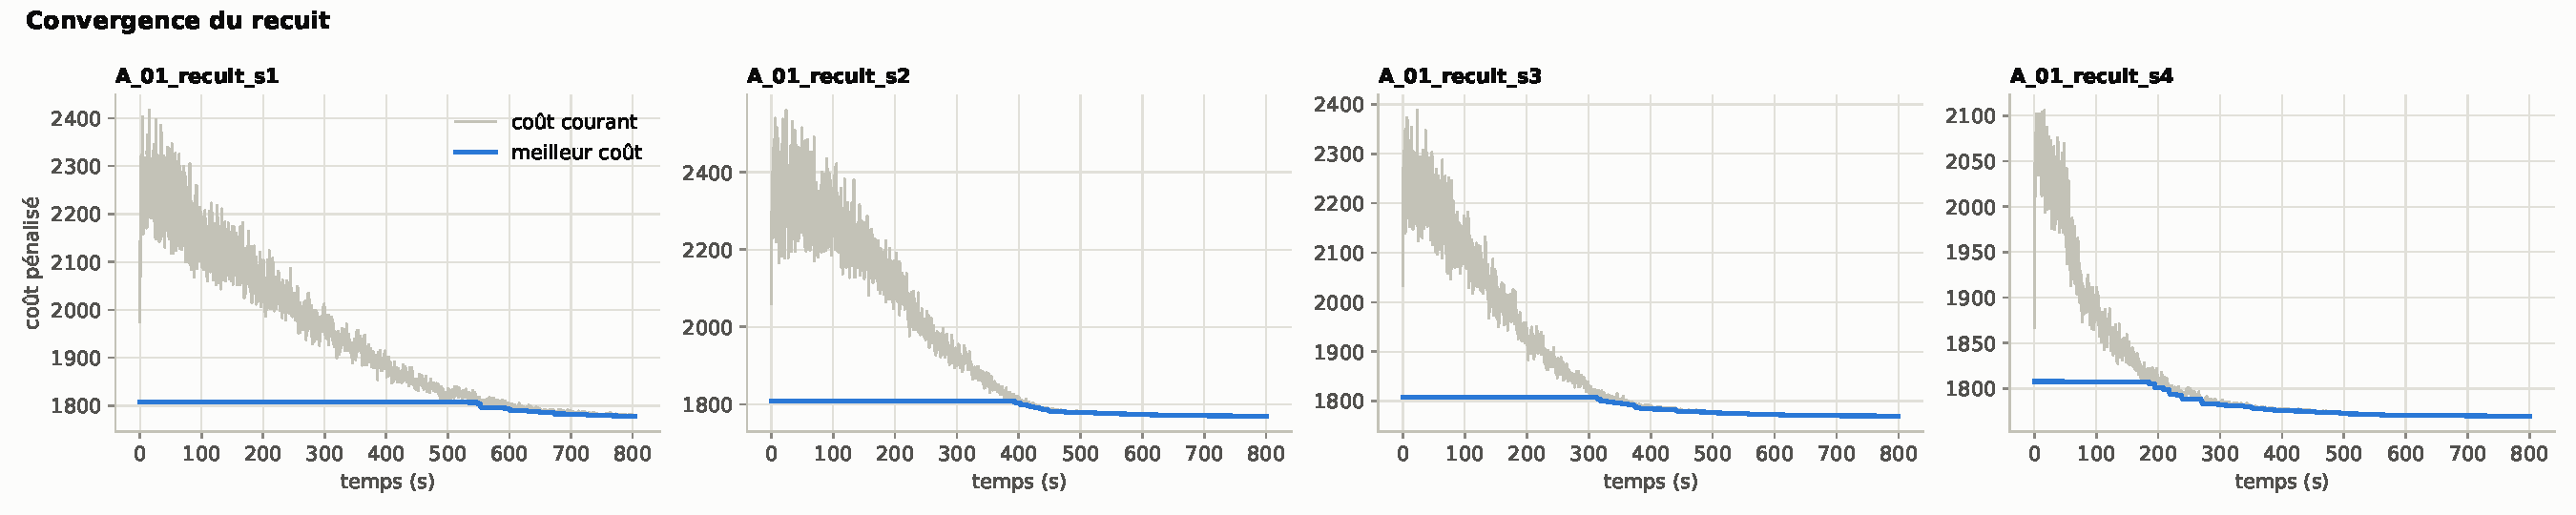
\includegraphics[width=\textwidth]{4_convergence.pdf}
\caption{Convergence du recuit sur A\_01, graines 1 à 4 : coût courant et meilleur coût.}
\label{fig:convergence}
\end{figure}

\begin{figure}[H]
\centering
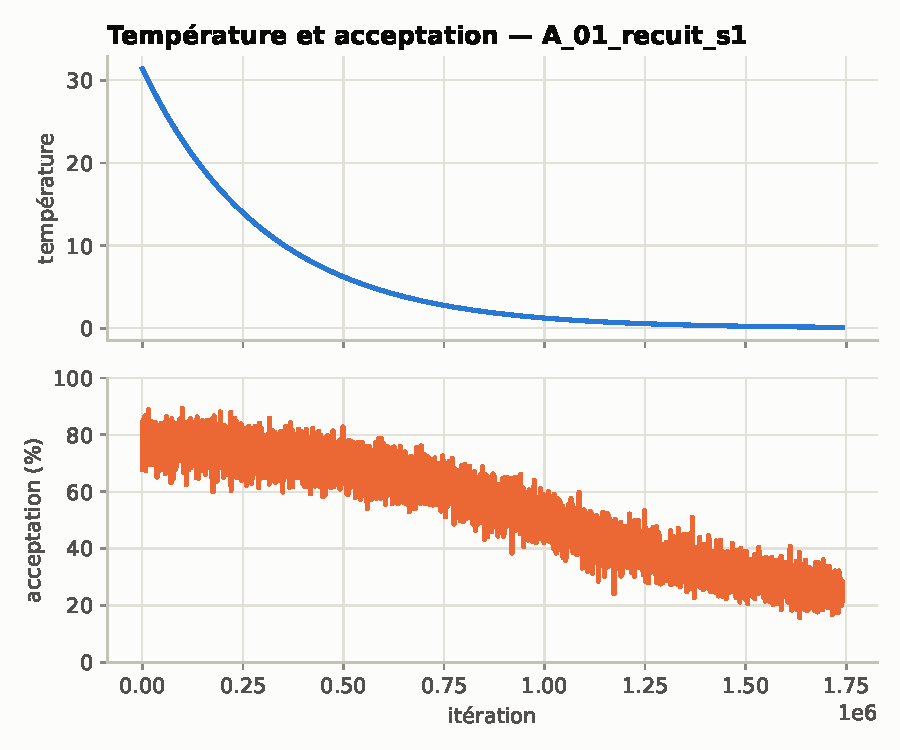
\includegraphics[width=0.55\textwidth]{5_temperature_acceptation.pdf}
\caption{Température et taux d'acceptation au fil des itérations (A\_01, graine 1).}
\label{fig:temperature}
\end{figure}

% ==================================================================== PLNE
\section{Programmation linéaire en nombres entiers}\label{sec:plne}

\subsection{Modèle}

La PLNE (\texttt{src/Plne.py}) utilise une variable binaire $x_{i,s}$ par intervention et par date
de début possible.
\begin{align*}
  & \textstyle\sum_{s \in \Sd_i} x_{i,s} = 1 && \forall i \in \I \\
  & r_{t,\omega} = \textstyle\sum_{i,s} r_i^{t,s,\omega} \, x_{i,s}, \qquad
    m_t = \frac{1}{S_t} \sum_\omega r_{t,\omega} && \text{(expressions linéaires)} \\
  & r_{t,\omega} \le Q_t + M_{t,\omega} \, y_{t,\omega}, \qquad
    \textstyle\sum_\omega y_{t,\omega} \le S_t - k_t, \qquad y_{t,\omega} \in \{0, 1\} && \text{(quantile)} \\
  & E_t \ge Q_t - m_t, \qquad E_t \ge 0 && \text{(excès)} \\
  & \underline{u}_c^t \le \textstyle\sum_{i,s} w_{i,c}^{t,s} \, x_{i,s} \le \overline{u}_c^t && \text{(ressources)} \\
  & \textstyle\sum_{s : i \text{ en cours en } t} x_{i,s} + \sum_{s : j \text{ en cours en } t} x_{j,s} \le 1
    && \text{(exclusions)} \\
  & \min \; \frac{1}{T} \textstyle\sum_t \big[ \alpha \, m_t + (1 - \alpha) \, E_t \big]
\end{align*}
Les contraintes de quantile imposent qu'au plus $S_t - k_t$ scénarios dépassent $Q_t$, donc qu'au
moins $k_t$ soient en dessous : $Q_t$ est supérieur ou égal au quantile, et l'objectif, qui pénalise
$E_t$, le ramène à sa valeur exacte. Le big-M vaut
$M_{t,\omega} = \sum_i \max_s r_i^{t,s,\omega} - \underline{Q}_t$, avec $\underline{Q}_t$ une borne
inférieure de $Q_t$ obtenue avec les contributions minimales. Avec un seul scénario, ou $\alpha = 1$,
il n'y a ni $Q$, ni $E$, ni $y$. Gurobi~\cite{gurobi} résout le modèle avec \texttt{MIPGap} $= 0$ (un
statut optimal est donc un optimum exact), en partant de la meilleure solution du recuit (MIP start).

\subsection{Faiblesse de la borne et coupes de quantile}

Sur les instances à plusieurs scénarios, la borne inférieure progresse lentement. Le cas extrême est
A\_02 (120 scénarios, 4,1 millions de non-zéros) : après 15 minutes, la borne vaut 2058 pour une
solution à 4672, soit un gap de 55,94\,\%. L'excès y pèse plus que le risque moyen
(\texttt{obj2} = 4943 contre \texttt{obj1} = 4401) mais, en relaxation, des $y_{t,\omega}$
fractionnaires suffisent à neutraliser les big-M : $Q_t$ n'est presque plus contraint et la borne ne
compte guère que la moyenne.

\paragraph{Essai : génération de contraintes sur les scénarios.} Gouvine~\cite{gouvine} propose de
résoudre un modèle restreint à un sous-ensemble $W_t$ de scénarios (relaxation valide : au moins
$|W_t| - (S_t - k_t)$ scénarios de $W_t$ sous $Q_t$), puis d'ajouter les scénarios qui dépassent $Q_t$
dans la solution obtenue. Sur A\_02, avec 9 scénarios par période, il faut 272 secondes pour résoudre
le modèle restreint à 1\,\% près, pour une borne de 1624 ; avec 13 scénarios, la borne atteint 2054,
le niveau du modèle complet. Le goulot n'est pas le nombre de binaires mais le big-M, et un petit
$W_t$ donne un rang de quantile trop bas. Nous avons abandonné cette piste.

\paragraph{Coupe retenue.} Au plus $S_t - k_t$ scénarios dépassent $Q_t$ ; tout ensemble $W$ de
$S_t - k_t + 1$ scénarios en contient donc au moins un sous $Q_t$. Comme chaque intervention n'a
qu'une date de début,
\[
  Q_t \;\ge\; \min_{\omega \in W} r_{t,\omega}
      \;\ge\; \sum_{i,s} \Big( \min_{\omega \in W} r_i^{t,s,\omega} \Big) \, x_{i,s}.
\]
Cette coupe est linéaire, valide pour toute solution entière, et n'ajoute aucune binaire. Elle est
forte quand les scénarios sont corrélés : sur la meilleure solution de A\_02, avec $W$ formé de ses
sept scénarios les plus hauts en chaque période, elle retrouve 96\,\% de l'excès (4763 sur 4943).

\paragraph{Mise en œuvre.}
\begin{enumerate}
  \item On résout la relaxation linéaire \emph{sans} les $y$ ni les big-M, où $Q_t$ n'est borné que par
        les coupes ; les premières coupes sont tirées de la solution de départ.
  \item Séparation : en chaque période, $W$ est formé des $S_t - k_t + 1$ scénarios les plus hauts de
        la solution relâchée ; la coupe est ajoutée si elle est violée, et on recommence jusqu'à ce
        qu'aucune ne le soit.
  \item Les coupes sont ajoutées à la PLNE complète, qui reste exacte, puis séparées de nouveau à
        chaque nœud de l'arbre de recherche (callback \texttt{cbCut} de Gurobi). La borne retenue est
        la meilleure des deux.
\end{enumerate}

\begin{table}[H]
\centering
\small
\caption{Effet des coupes de quantile sur A\_02 (départ : meilleur recuit).}
\label{tab:coupes}
\begin{tabular}{lrrr}
\toprule
Configuration & Borne & Solution & Gap certifié \\
\midrule
Modèle seul, 900 s & 2058,39 & 4672,13 & 55,94\,\% \\
Relaxation + 351 coupes (8 s) & 4561,96 & -- & -- \\
Coupes + PLNE, 300 s, sans coupes aux nœuds & 4574,58 & 4672,13 & 2,09\,\% \\
Coupes + PLNE, 300 s, avec coupes aux nœuds & 4582,43 & 4672,13 & 1,92\,\% \\
\textbf{Coupes + PLNE, 900 s} & \textbf{4610,21} & \textbf{4671,94} & \textbf{1,32\,\%} \\
\bottomrule
\end{tabular}
\end{table}

La relaxation avec coupes, résolue en 8 secondes, donne déjà une borne bien meilleure que 15 minutes
de branch-and-bound sur le modèle seul (tableau~\ref{tab:coupes}). Au bout de 900 secondes, la borne
certifie que la meilleure valeur du challenge (4671,38) est à moins de 1,31\,\% de l'optimum, et la
PLNE améliore aussi la solution du recuit (4672,13 puis 4671,94), ce qu'elle ne faisait pas sans les
coupes.

% =============================================================== protocole
\section{Protocole expérimental}\label{sec:protocole}

\begin{itemize}
  \item \textbf{Budget.} Recuit et PLNE disposent du temps du challenge, 15 minutes par instance
        (lecture du fichier JSON non comprise pour le recuit, construction du modèle comprise pour la
        PLNE). Le glouton s'exécute une fois, et nous relevons son temps.
  \item \textbf{Graines.} Le recuit est lancé avec cinq graines (1 à 5) sur chaque instance ; nous
        donnons la moyenne, l'écart-type et la meilleure valeur.
  \item \textbf{Juge.} Toutes les solutions sont vérifiées par le checker officiel du
        challenge~\cite{depot}.
  \item \textbf{Référence.} Les écarts sont mesurés à la meilleure valeur trouvée pendant la
        qualification du challenge (15 minutes)~\cite{qualif}.
  \item \textbf{Réglage et évaluation.} A\_06, A\_09 et A\_13 ont servi au réglage du recuit : elles
        sont présentées à part, et les moyennes qui servent de conclusion portent sur les douze autres
        instances. Le profil de performance (figure~\ref{fig:profil}) ne porte que sur ces douze
        instances.
  \item \textbf{Machine.} Intel Core i7-1185G7 (4 cœurs, 8 fils), 15 Go de mémoire ; Python 3.12,
        NumPy 2.5, Gurobi 13.0 (licence académique). Six exécutions du recuit en parallèle ; une PLNE
        à la fois, sur tous les cœurs, avec une limite mémoire de 8 Go.
\end{itemize}

% ================================================================ résultats
\section{Résultats}\label{sec:resultats}

\subsection{Tableau comparatif}

Le tableau~\ref{tab:principal} rassemble les trois méthodes ; il est produit par
\texttt{src/tableau.py} à partir de \texttt{results/results.csv}. Les 75 exécutions du recuit sont
réalisables, de même que les 15 solutions de la PLNE.

\begin{table}[H]
\centering
\caption{Comparaison au temps du challenge. Entre parenthèses : écart à la référence ; en gras :
référence atteinte (écart inférieur à 0,001\,\%). Gap certifié : (PLNE $-$ borne) / PLNE.
$^\dagger$ : borne obtenue avec les coupes de quantile. Les moyennes portent sur les écarts.}
\label{tab:principal}
\scriptsize
\setlength{\tabcolsep}{4pt}
% Généré par python src/tableau.py : ne pas modifier à la main
\begin{tabular}{lrrrrrrr}
\toprule
Instance & Référence & Glouton & \makecell{Recuit\\ moy. $\pm$ $\sigma$} & \makecell{Recuit\\ meilleur} & PLNE & \makecell{Borne\\ PLNE} & \makecell{Gap\\ certifié} \\
\midrule
\multicolumn{8}{l}{\textit{Instances hors réglage (12)}} \\
\midrule
A\_01 & 1767,82 & \makecell{1807,83\\ \footnotesize(2,26 \%)} & \makecell{1769,81 $\pm$ 0,73\\ \footnotesize(0,11 \%)} & \makecell{1769,24\\ \footnotesize(0,08 \%)} & \makecell{\textbf{1767,82}\\ \footnotesize(0)} & 1767,82 & 0 (optimal) \\
A\_02 & 4671,38 & \makecell{4685,07\\ \footnotesize(0,29 \%)} & \makecell{4673,54 $\pm$ 1,09\\ \footnotesize(0,05 \%)} & \makecell{4672,13\\ \footnotesize(0,02 \%)} & \makecell{4671,94\\ \footnotesize(0,01 \%)} & 4610,21$^\dagger$ & 1,32 \% \\
A\_03 & 848,18 & \makecell{850,80\\ \footnotesize(0,31 \%)} & \makecell{849,67 $\pm$ 1,32\\ \footnotesize(0,18 \%)} & \makecell{\textbf{848,18}\\ \footnotesize(0)} & \makecell{\textbf{848,18}\\ \footnotesize(0)} & 848,18 & 0 (optimal) \\
A\_04 & 2085,88 & \makecell{2173,63\\ \footnotesize(4,21 \%)} & \makecell{2103,37 $\pm$ 6,20\\ \footnotesize(0,84 \%)} & \makecell{2093,37\\ \footnotesize(0,36 \%)} & \makecell{\textbf{2085,88}\\ \footnotesize(0)} & 2085,88 & 0 (optimal) \\
A\_05 & 635,22 & \makecell{639,87\\ \footnotesize(0,73 \%)} & \makecell{636,01 $\pm$ 0,53\\ \footnotesize(0,12 \%)} & \makecell{635,37\\ \footnotesize(0,02 \%)} & \makecell{635,37\\ \footnotesize(0,02 \%)} & 593,49 & 6,59 \% \\
A\_07 & 2272,78 & \makecell{\textbf{2272,78}\\ \footnotesize(0)} & \makecell{2272,78 $\pm$ 0,00\\ \footnotesize(0)} & \makecell{\textbf{2272,78}\\ \footnotesize(0)} & \makecell{\textbf{2272,78}\\ \footnotesize(0)} & 2272,78 & 0 (optimal) \\
A\_08 & 744,29 & \makecell{745,83\\ \footnotesize(0,21 \%)} & \makecell{744,29 $\pm$ 0,00\\ \footnotesize(0)} & \makecell{\textbf{744,29}\\ \footnotesize(0)} & \makecell{\textbf{744,29}\\ \footnotesize(0)} & 700,11 & 5,94 \% \\
A\_10 & 2994,85 & \makecell{2997,25\\ \footnotesize(0,08 \%)} & \makecell{2994,97 $\pm$ 0,16\\ \footnotesize(0,004 \%)} & \makecell{\textbf{2994,85}\\ \footnotesize(0)} & \makecell{\textbf{2994,85}\\ \footnotesize(0)} & 2994,85 & 0 (optimal) \\
A\_11 & 495,26 & \makecell{501,62\\ \footnotesize(1,29 \%)} & \makecell{495,44 $\pm$ 0,20\\ \footnotesize(0,04 \%)} & \makecell{495,27\\ \footnotesize(0,003 \%)} & \makecell{495,27\\ \footnotesize(0,002 \%)} & 460,59 & 7,00 \% \\
A\_12 & 789,63 & \makecell{792,00\\ \footnotesize(0,30 \%)} & \makecell{789,73 $\pm$ 0,18\\ \footnotesize(0,01 \%)} & \makecell{\textbf{789,63}\\ \footnotesize(0)} & \makecell{\textbf{789,63}\\ \footnotesize(0)} & 789,63 & 0 (optimal) \\
A\_14 & 2264,12 & \makecell{2537,23\\ \footnotesize(12,06 \%)} & \makecell{2321,53 $\pm$ 9,13\\ \footnotesize(2,54 \%)} & \makecell{2312,69\\ \footnotesize(2,14 \%)} & \makecell{2312,36\\ \footnotesize(2,13 \%)} & 2080,06 & 10,05 \% \\
A\_15 & 2268,57 & \makecell{2547,18\\ \footnotesize(12,28 \%)} & \makecell{2323,28 $\pm$ 17,03\\ \footnotesize(2,41 \%)} & \makecell{2314,94\\ \footnotesize(2,04 \%)} & \makecell{2314,92\\ \footnotesize(2,04 \%)} & 2071,06 & 10,53 \% \\
\textbf{Moyenne} &  & 2,83 \% & 0,52 \% & 0,39 \% & 0,35 \% &  & 3,45 \% \\
\midrule
\multicolumn{8}{l}{\textit{Instances de réglage du recuit (3)}} \\
\midrule
A\_06 & 590,62 & \makecell{641,15\\ \footnotesize(8,55 \%)} & \makecell{601,23 $\pm$ 7,31\\ \footnotesize(1,80 \%)} & \makecell{594,69\\ \footnotesize(0,69 \%)} & \makecell{\textbf{590,62}\\ \footnotesize(0)} & 590,62 & 0 (optimal) \\
A\_09 & 1507,28 & \makecell{1586,19\\ \footnotesize(5,23 \%)} & \makecell{1507,28 $\pm$ 0,00\\ \footnotesize(0)} & \makecell{\textbf{1507,28}\\ \footnotesize(0)} & \makecell{\textbf{1507,28}\\ \footnotesize(0)} & 1507,28 & 0 (optimal) \\
A\_13 & 1998,66 & \makecell{2012,72\\ \footnotesize(0,70 \%)} & \makecell{2000,53 $\pm$ 1,35\\ \footnotesize(0,09 \%)} & \makecell{1999,00\\ \footnotesize(0,02 \%)} & \makecell{1998,84\\ \footnotesize(0,009 \%)} & 1998,36 & 0,02 \% \\
\textbf{Moyenne} &  & 4,83 \% & 0,63 \% & 0,23 \% & 0,003 \% &  & 0,008 \% \\
\bottomrule
\end{tabular}

\end{table}

\begin{itemize}
  \item \textbf{Glouton.} En moyenne à 2,83\,\% de la référence sur les instances hors réglage. Il
        est bon sur les instances faciles (0,3\,\% ou moins sur A\_02, A\_03, A\_08, A\_10, A\_12, et la
        référence sur A\_07), mais s'éloigne quand il a dû réparer des violations (A\_04 : 4,21\,\% ;
        A\_14 et A\_15 : 12\,\%).
  \item \textbf{Recuit.} En moyenne à 0,52\,\% hors réglage, et 0,39\,\% pour la meilleure des cinq
        graines. La meilleure graine atteint la référence sur six instances (A\_03, A\_07, A\_08, A\_09,
        A\_10, A\_12) et en est à moins de 0,1\,\% sur cinq autres. Les points faibles sont A\_14 et
        A\_15 (2\,\% environ), où le glouton partait de 12\,\%.
  \item \textbf{Réglage.} Sur les instances de réglage, l'écart moyen du recuit (0,63\,\%) n'est pas
        meilleur que hors réglage (0,52\,\%) : le réglage n'a pas favorisé ses propres instances, ce qui
        est cohérent avec le choix de garder les valeurs par défaut.
  \item \textbf{PLNE.} Optimum prouvé sur huit instances (A\_01, A\_03, A\_04, A\_06, A\_07, A\_09, A\_10,
        A\_12), toutes égales à la référence ; sur A\_01, A\_04 et A\_06, la PLNE améliore la meilleure
        graine du recuit jusqu'à l'optimum (A\_06 : 594,69 puis 590,62). Ailleurs, elle garde à peu près
        la solution de départ, et son apport est la borne.
\end{itemize}

\subsection{Comparaison par instance}

La figure~\ref{fig:methodes} montre l'écart de la meilleure solution de chaque méthode, la
figure~\ref{fig:dispersion} la dispersion du recuit entre graines. Les petites instances (A\_07 à
A\_12) donnent le même résultat pour toutes les graines ; A\_04, A\_06, A\_14 et A\_15 sont les plus
dispersées (écart-type de 6 à 17), et y lancer plusieurs graines est utile.

\begin{figure}[H]
\centering
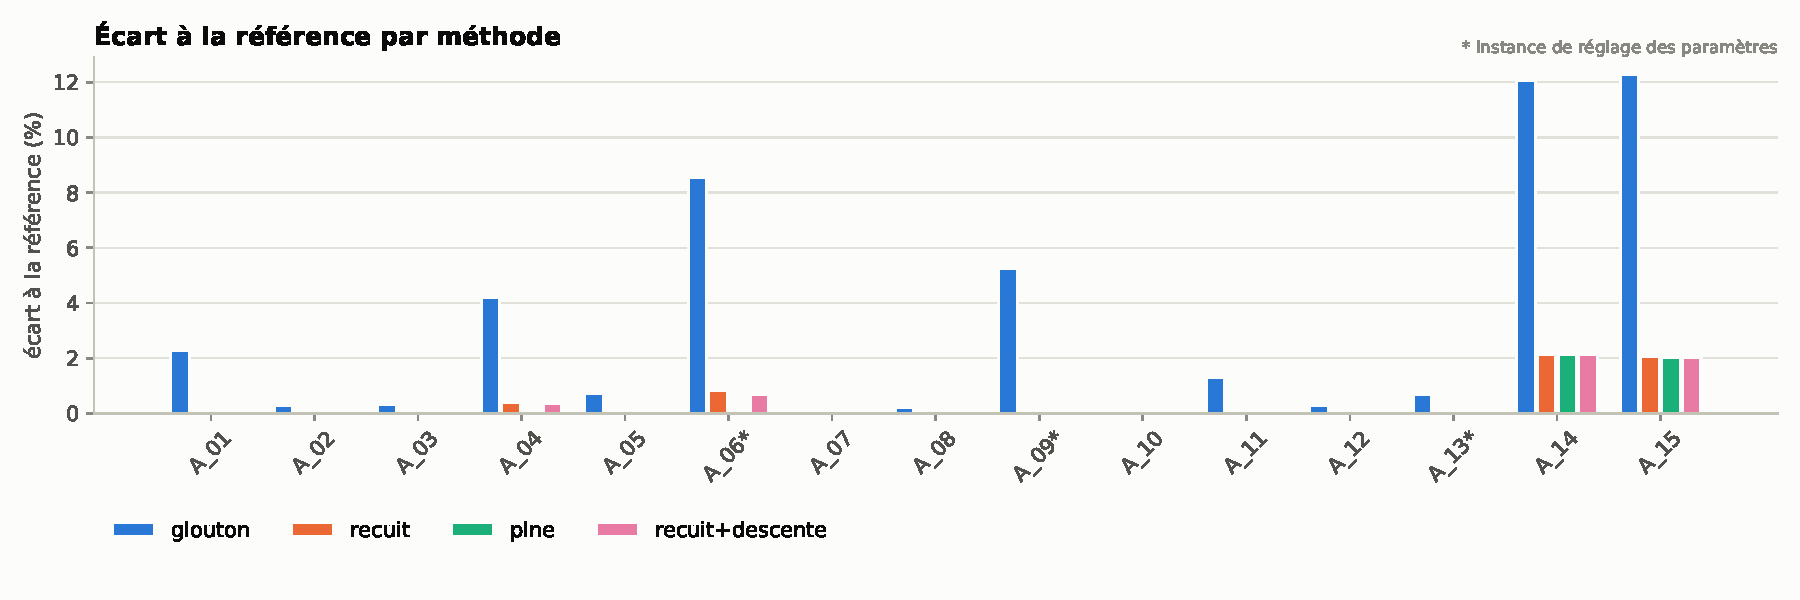
\includegraphics[width=\textwidth]{1_methodes.pdf}
\caption{Écart à la référence de la meilleure solution de chaque méthode (* : instance de réglage).}
\label{fig:methodes}
\end{figure}

\begin{figure}[H]
\centering
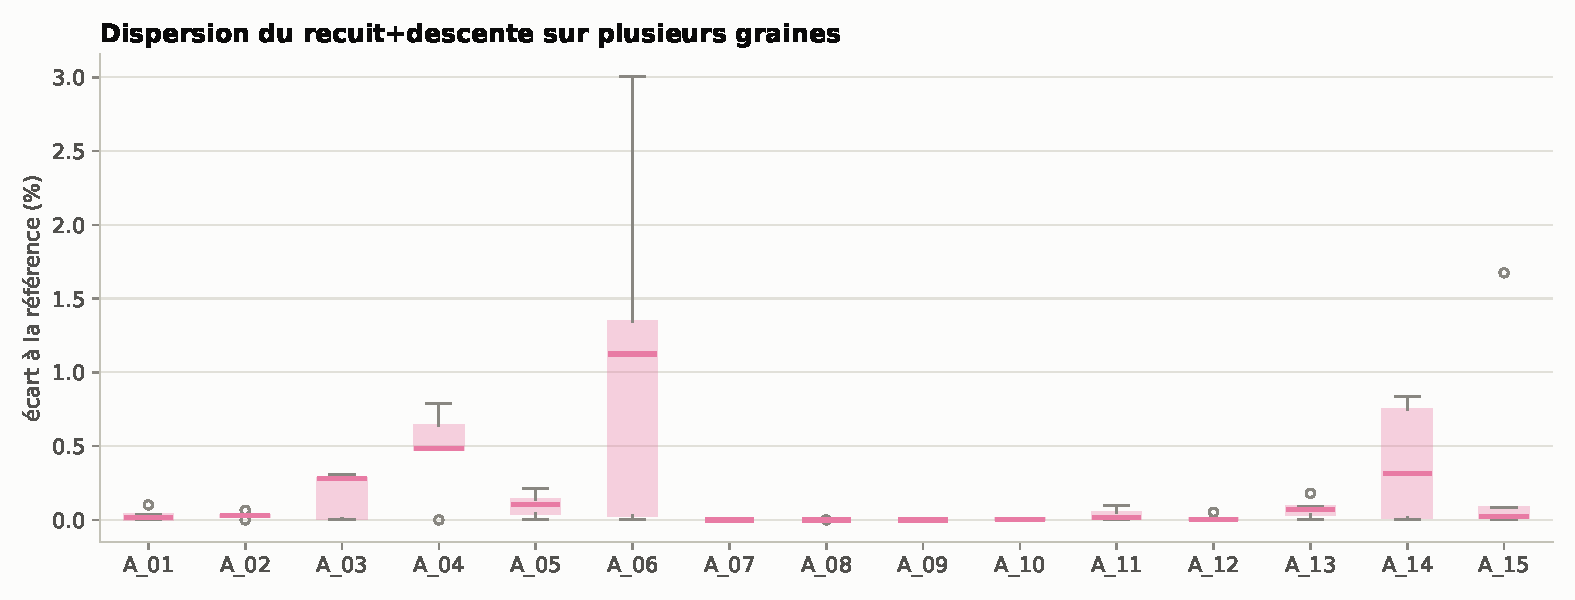
\includegraphics[width=\textwidth]{2_dispersion_recuit_descente.pdf}
\caption{Dispersion du recuit suivi de la descente sur les cinq graines.}
\label{fig:dispersion}
\end{figure}

\paragraph{Apport de la descente finale.} Sur les 75 exécutions, la descente améliore la solution du
recuit dans 52 cas, de 0,13\,\% en moyenne ; le gain dépasse 0,8\,\% sur quelques exécutions (A\_04,
A\_14, A\_06, et 2,69\,\% sur A\_15, graine 4), quand le recuit s'est arrêté loin d'un minimum local.
L'essentiel du gain sur le glouton vient du recuit (figure~\ref{fig:etapes} en annexe).

\subsection{Effet de la taille}

\begin{figure}[H]
\centering
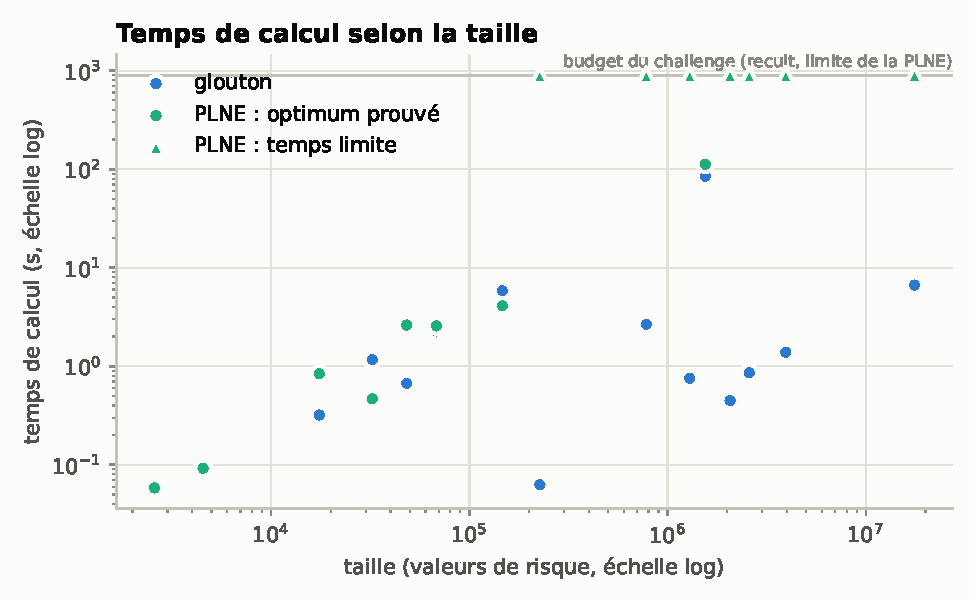
\includegraphics[width=0.49\textwidth]{12a_temps_taille.pdf}\hfill
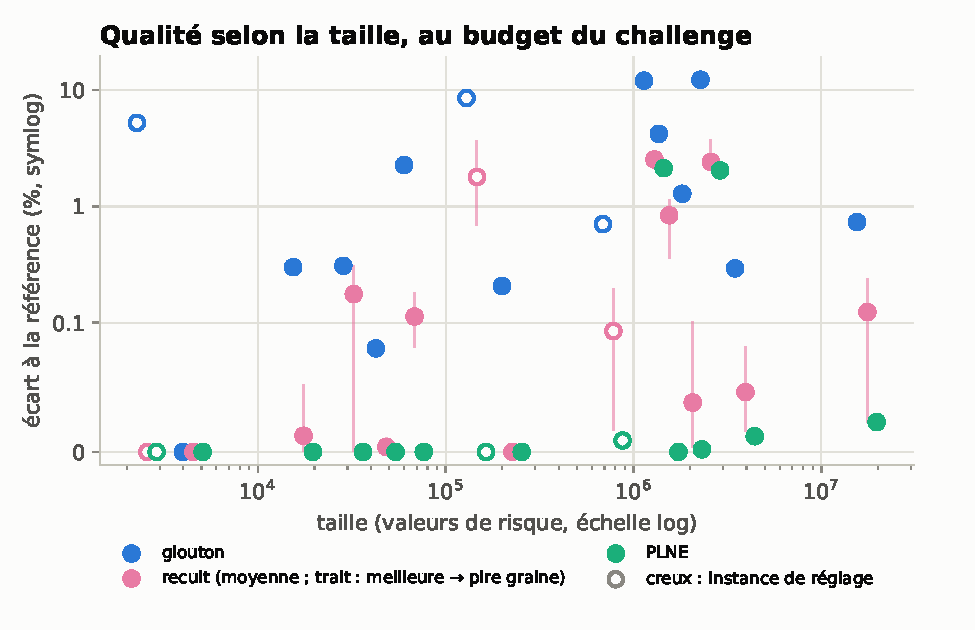
\includegraphics[width=0.49\textwidth]{12b_ecart_taille.pdf}
\caption{À gauche : temps du glouton et de la PLNE selon la taille (échelle log-log). À droite :
écart à la référence selon la taille, au budget du challenge ; trait du recuit : de la meilleure à la
pire graine ; marqueurs creux : instances de réglage.}
\label{fig:taille}
\end{figure}

La PLNE prouve l'optimum en quelques secondes jusqu'à environ $1{,}5 \cdot 10^5$ valeurs de risque,
et sur A\_04 (1,5 million de valeurs, mais un seul scénario) en 112 secondes ; à partir de A\_08
($2{,}3 \cdot 10^5$ valeurs, 693 scénarios), elle atteint le temps limite (figure~\ref{fig:taille}).
Le nombre de scénarios compte donc plus que la taille brute : le quantile est la vraie difficulté du
modèle. L'écart du recuit ne croît pas avec la taille ; il dépend surtout des instances où le glouton
part de loin.

\subsection{Profil de performance}

Le profil de performance de Dolan et Moré (figure~\ref{fig:profil}) donne, pour chaque méthode, la
part des instances où elle est à moins de $x$\,\% de la meilleure des méthodes comparées. Sur les douze
instances hors réglage, la meilleure graine du recuit est toujours à moins de 0,4\,\%, la moyenne des
graines à moins de 0,9\,\% et le glouton jusqu'à 10\,\%. La PLNE est en tête sur toutes les instances,
mais \emph{par construction} : elle part de la meilleure graine du recuit et ne peut pas faire moins
bien. Ce profil compare donc le recuit au glouton ; il ne montre pas que la PLNE seule ferait mieux.

\begin{figure}[H]
\centering
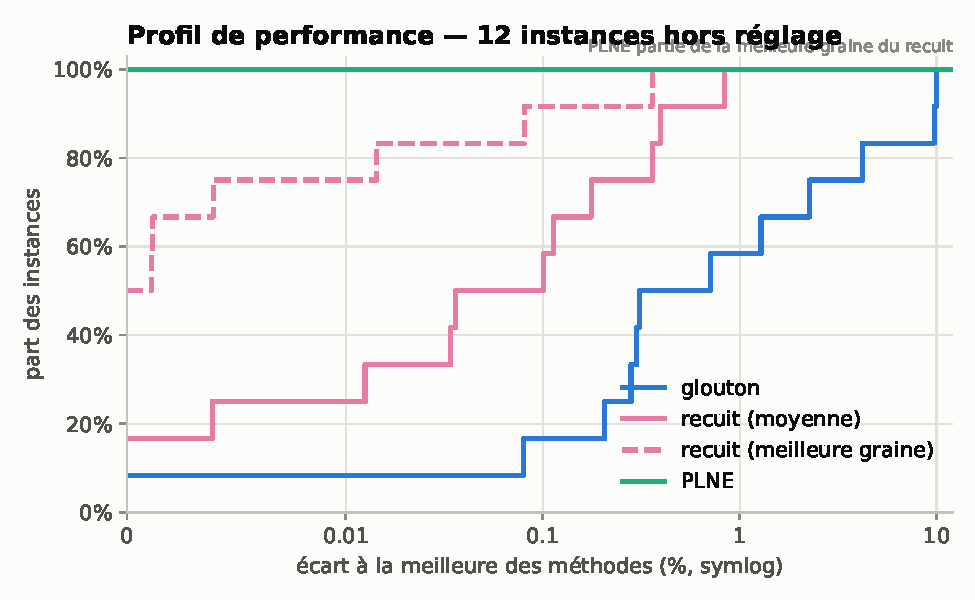
\includegraphics[width=0.6\textwidth]{13_profil_performance.pdf}
\caption{Profil de performance sur les douze instances hors réglage.}
\label{fig:profil}
\end{figure}

% =============================================================== discussion
\section{Discussion et limites}\label{sec:discussion}

\begin{itemize}
  \item \textbf{Rôles complémentaires.} Le glouton donne en quelques secondes une solution réalisable
        à quelques pourcents ; le recuit est le meilleur compromis au budget du challenge ; la PLNE est
        exacte sur les instances à peu de scénarios, et sa borne mesure la qualité des autres
        solutions.
  \item \textbf{Réglage limité.} Deux graines et 120 secondes par configuration, un facteur à la fois :
        le bruit entre graines empêche de départager des variantes à moins de 1\,\%. Un réglage plus
        fiable demanderait plus de graines, le budget complet, et un plan qui teste les interactions.
  \item \textbf{Cinq graines} au lieu des dix prévues, faute de temps de calcul (la campagne finale
        prend déjà 3 h 30 sur six cœurs).
  \item \textbf{PLNE dépendante du recuit.} Le MIP start vient de la meilleure graine : la qualité des
        solutions PLNE n'est pas celle d'une PLNE seule. Les coupes de quantile n'ont été évaluées au
        budget du challenge que sur A\_02 ; les autres instances limitées par le temps (A\_05, A\_08,
        A\_11, A\_13, A\_14, A\_15, gaps de 0,02 à 10,5\,\%) restent à traiter.
  \item \textbf{Instances B} non évaluées : le recuit termine la réparation de B\_01, que le glouton
        laisse avec de petits dépassements, mais aucune campagne n'a été menée sur l'ensemble B.
  \item \textbf{Glouton.} La version randomisée multi-départ (GRASP) et la comparaison des critères de
        tri n'ont pas été menées ; le score de difficulté est utilisé avec un seul jeu de poids.
\end{itemize}

% =============================================================== conclusion
\section{Conclusion}

Sur les 15 instances A du challenge ROADEF/EURO 2020, au temps du challenge, le recuit simulé
suivi d'une descente ramène l'écart moyen à la meilleure valeur connue de 2,83\,\% (glouton) à
0,52\,\% sur les douze instances qui n'ont pas servi à le régler, avec 75 exécutions sur 75
réalisables. La PLNE prouve l'optimum de huit instances et certifie la qualité des autres solutions.
Une coupe linéaire simple sur le quantile, valide pour toute solution entière, renforce nettement sa
borne quand les scénarios sont corrélés : sur A\_02, le gap certifié passe de 55,94\,\% à 1,32\,\%.

Les suites naturelles sont d'appliquer ces coupes aux six autres instances limitées par le temps,
d'en tirer une borne pour guider le recuit, et d'évaluer les méthodes sur les instances B, plus
grandes.

% ============================================================ bibliographie
\begin{thebibliography}{9}

\bibitem{sujet} P. Tournebise, M. Ruiz, P. Pancia (RTE). \emph{ROADEF Challenge RTE: Grid
operation-based outage maintenance planning}. Sujet du challenge ROADEF/EURO 2020.
\url{https://github.com/rte-france/challenge-roadef-2020}

\bibitem{depot} RTE. Dépôt officiel du challenge ROADEF/EURO 2020 (instances et checker).
\url{https://github.com/rte-france/challenge-roadef-2020} ;
\url{https://www.roadef.org/challenge/2020/en/}

\bibitem{qualif} ROADEF/EURO Challenge 2020. \emph{Qualification results}.
\url{https://roadef.org/challenge/2020/en/qualifresult.php}, consulté le 8 octobre 2026.

\bibitem{gouvine} G. Gouvine. \emph{Mixed-Integer Programming decomposition for stochastic
programming with quantiles}. arXiv:2111.01047v2 [math.OC], 2023.

\bibitem{kirkpatrick} S. Kirkpatrick, C. D. Gelatt, M. P. Vecchi. Optimization by Simulated
Annealing. \emph{Science}, 220(4598):671--680, 1983.

\bibitem{gurobi} Gurobi Optimization, LLC. \emph{Gurobi Optimizer Reference Manual}.
\url{https://docs.gurobi.com}

\end{thebibliography}

% ================================================================== annexes
\appendix
\section{Figures complémentaires}

\begin{figure}[H]
\centering
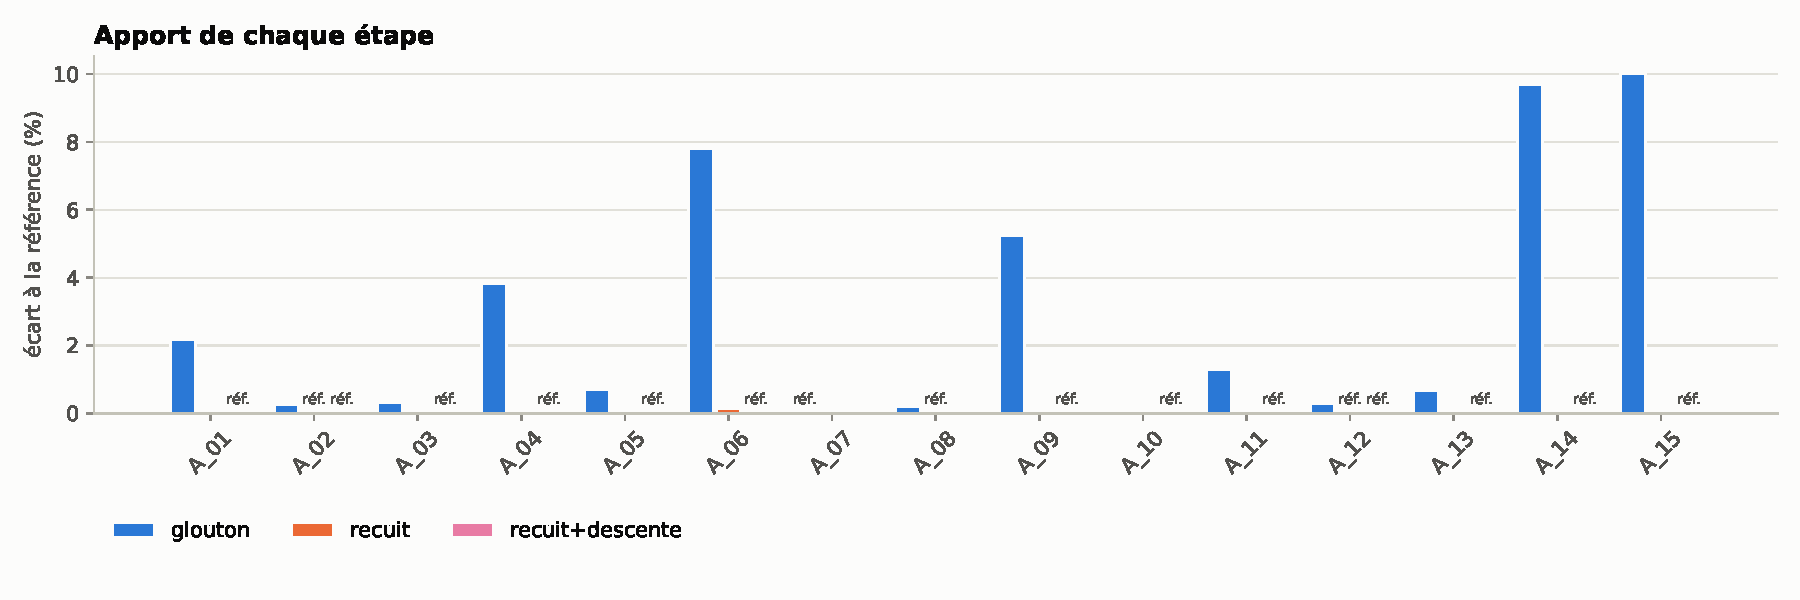
\includegraphics[width=\textwidth]{8_apport_etapes.pdf}
\caption{Apport de chaque étape : glouton, recuit, recuit suivi de la descente (meilleure graine).}
\label{fig:etapes}
\end{figure}

\begin{figure}[H]
\centering
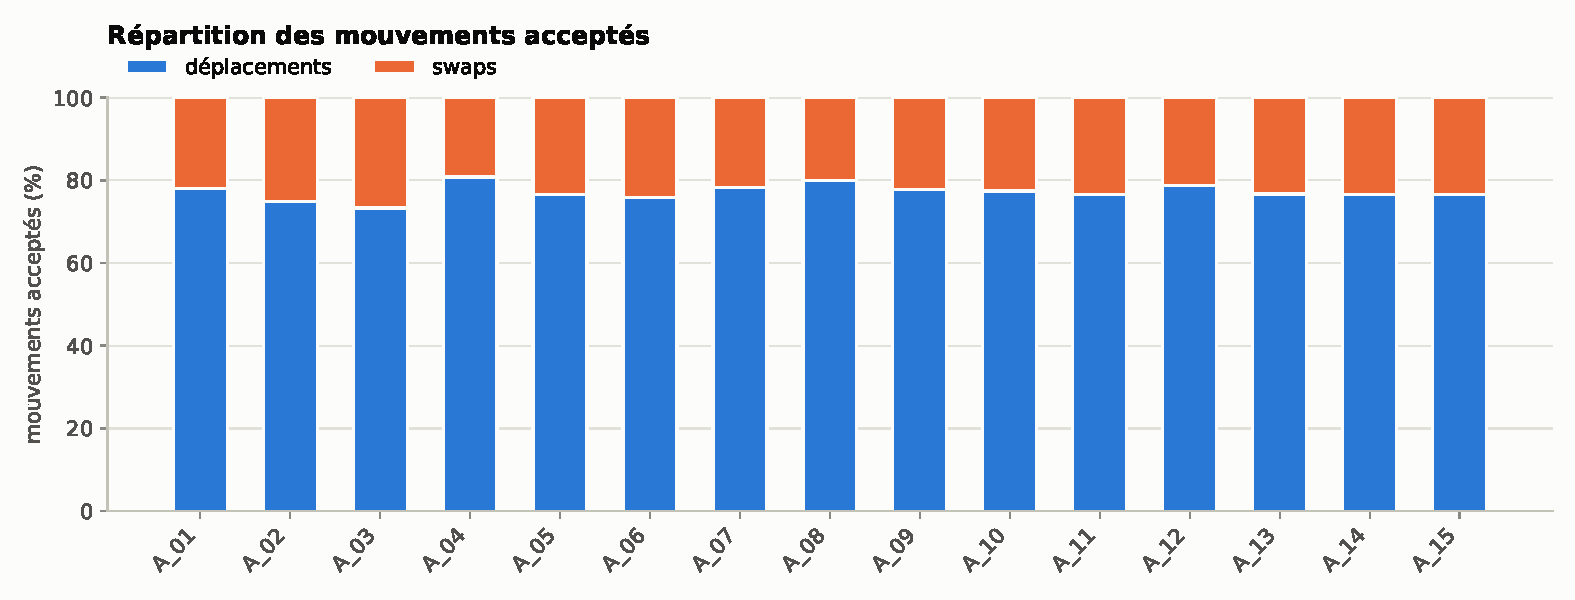
\includegraphics[width=\textwidth]{6_mouvements.pdf}
\caption{Part des déplacements et des swaps parmi les mouvements acceptés (graines cumulées).}
\label{fig:mouvements}
\end{figure}

\begin{figure}[H]
\centering
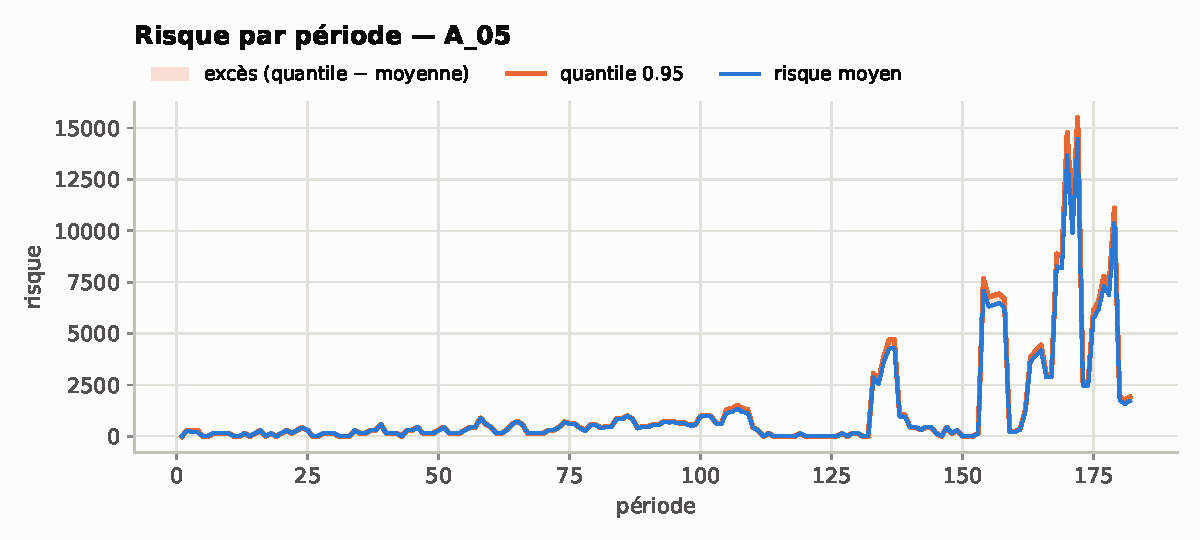
\includegraphics[width=0.8\textwidth]{11_risque_A_05.pdf}
\caption{Risque moyen et quantile 0,95 par période, meilleure solution du recuit sur A\_05 (graine 2, 635,37) ; l'écart
entre les deux courbes est le terme d'excès.}
\label{fig:risque}
\end{figure}

\begin{figure}[H]
\centering
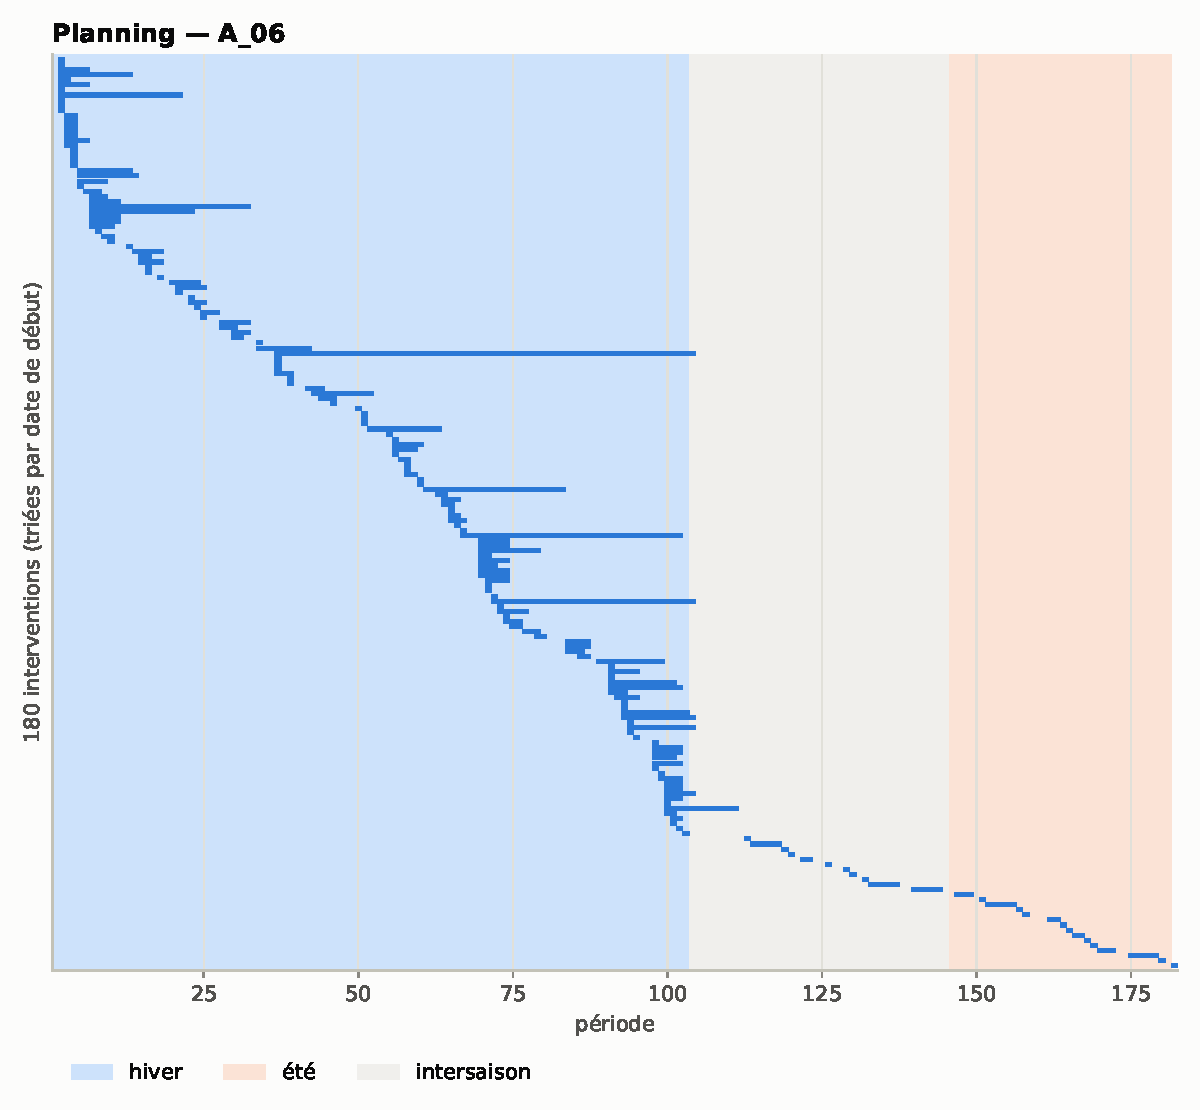
\includegraphics[width=0.7\textwidth]{9_gantt_A_06.pdf}
\caption{Planning de la meilleure solution du recuit sur A\_06 (594,69), saisons en fond.}
\label{fig:gantt}
\end{figure}

\section{Reproduire les résultats}

\begin{verbatim}
make install                                  # environnement Python (.venv)
python src/campagne.py finale                 # recuit : 15 instances A x 5 graines
python src/campagne.py plne                   # PLNE, départ : meilleur recuit
python src/campagne.py plne --coupes --instances A_02
make tableau                                  # results/tableau.md, .csv, .tex
make graphes                                  # results/figures/
\end{verbatim}

Les solutions sont dans \texttt{solutions/}, et chacune peut être vérifiée avec
\texttt{make check INSTANCE=A\_set/A\_01.json SOLUTION=solutions/A\_01\_plne.txt}.

\end{document}
